\documentclass[11pt]{article}

% Page layout.
\usepackage[margin=1in]{geometry}

% Figures, tables, and hyperlinks.
\usepackage{graphicx}
\usepackage{booktabs}
\usepackage{float}
\usepackage[hidelinks]{hyperref}

% Folder containing the exported figures.
\graphicspath{{figures/}}

% Paragraph formatting and flexible line spacing.
\setlength{\parindent}{0pt}
\setlength{\parskip}{6pt}
\setlength{\emergencystretch}{3em}

% Title information.
\title{Exploratory Analysis of MMP11 and SCARA5 Counts\\
in Breast Cancer}
\author{Jamie Ghossein}
\date{October 18, 2026}

\begin{document}

\maketitle

\section{Introduction}

This project explores RNA-seq gene counts and sample metadata
from The Cancer Genome Atlas Breast Invasive Carcinoma
(TCGA-BRCA) cohort, whose data are available through the
National Cancer Institute's Genomic Data Commons
\cite{gdc}. I used the course-provided count matrix and
metadata files. The matrix contains 60,660 genes across
1,231 samples: 1,111 primary tumors, 113 normal tissue
samples, and seven metastatic samples.

To guide gene selection, I first explored genes with large
observed differences between normal and primary tumor
samples. An exploratory heatmap helped me examine these
patterns across individual samples. I selected
\textit{MMP11} as my main gene because it generally showed
higher expression in primary tumors, and \textit{SCARA5}
as a comparison gene because it showed the opposite pattern.

\textit{MMP11} encodes matrix metallopeptidase 11, also called
stromelysin-3. It was originally identified in stromal cells
surrounding invasive breast carcinomas, making it relevant
to the study of the tumor microenvironment \cite{basset1990}.
\textit{SCARA5} encodes scavenger receptor class A member 5.
Previous research reported reduced SCARA5 expression in
breast tumors compared with matched noncancerous tissue
\cite{ulker2018}.

My objective was to describe the distributions of these
genes' counts and compare patterns across tissue types.
Following peer feedback, I highlighted the metastatic
samples to examine their positions relative to normal
and primary tumor samples. I also added PAM50 molecular
subtype annotations to the heatmap to provide further
context for variation among primary tumors.

Because gene selection followed exploration of this same
dataset, the findings are descriptive and exploratory.


\section{Methods}

\subsection{Data preparation}

I imported the course-provided count matrix and sample
metadata into R. Rows in the count matrix represent genes,
and columns represent samples. I matched the sample
barcodes in the metadata to the corresponding count
columns so that each sample's gene counts were associated
with the correct tissue type.

The analysis included 113 normal tissue samples,
1,111 primary tumor samples, and seven metastatic samples.
I extracted counts for \textit{MMP11}
(ENSG00000099953.10) and \textit{SCARA5}
(ENSG00000168079.17) for the two-gene comparisons.

\subsection{Exploratory gene selection}

For the initial comparison of normal and primary tumor
samples, I converted raw counts to counts per million
(CPM) by dividing each count by its sample's total count
across all genes and multiplying by one million.
I retained genes with at least one CPM in at least
10 samples and transformed their values using
$\log_2(\mathrm{CPM}+1)$.

I calculated the difference between the median transformed
values in primary tumor and normal tissue samples for
each retained gene. I ranked genes by the absolute size
of this difference and explored the top 20 candidates
using a heatmap. This exploration guided my selection
of \textit{MMP11} and \textit{SCARA5}.

\subsection{Summary statistics and visualizations}

For each selected gene, I calculated the sample size,
mean, median, standard deviation, minimum, and maximum
of the raw counts across all samples.

I used a histogram to examine the distribution of
\textit{MMP11} counts within each tissue group, a scatter
plot to examine the relationship between the two genes,
and box plots to compare their distributions across
tissue types. These plots used
$\log_{10}(\mathrm{raw\ count}+1)$ to make the wide range
of counts easier to display. Adding one allowed samples
with zero counts to remain in the plots.
This transformation does not normalize counts for
differences in sequencing depth.

Following peer feedback, I highlighted the seven
metastatic samples as orange triangles in the scatter
plot. I also displayed individual metastatic samples
on the box plots because this group was small.

As an additional plot type, I created empirical
cumulative distribution function (ECDF) plots using
\texttt{stat\_ecdf()} in ggplot2 \cite{ecdf}.
At each count value, an ECDF shows the proportion
of samples with values at or below that value.
These plots allowed me to compare distributions
across tissue groups without choosing histogram bins.

\subsection{Heatmap}

The final heatmap included 10 unique genes:
\textit{MMP11}, \textit{SCARA5}, and eight additional
genes from the exploratory candidate list.
For these genes, I calculated CPM using sample totals
from the complete count matrix, applied
$\log_2(\mathrm{CPM}+1)$, and standardized each gene
across samples using a row z-score.

For each gene, the z-score was calculated by subtracting
its mean transformed value across samples and dividing
by its standard deviation. Positive values therefore
indicate values above that gene's mean, while negative
values indicate values below its mean.

I grouped samples by tissue type and used hierarchical
clustering to organize genes and samples within each
tissue group. Annotation bars identified tissue type
and the PAM50 molecular subtype recorded in the metadata.
Missing subtype information was displayed as
``Not available.''

\subsection{Software and scope}

I performed the analysis using R version 4.6.1.
Data preparation used tidyverse 2.0.0, including
dplyr 1.2.1, tidyr 1.3.2, and tibble 3.3.1.
Plots used ggplot2 4.0.3 and scales 1.4.0.
The heatmap used ComplexHeatmap 2.28.0 and
circlize 0.4.18.
The accompanying R Markdown document used
knitr 1.51 and rmarkdown 2.32.

The analysis was descriptive and exploratory.
I did not perform hypothesis tests or a formal
differential expression analysis. Samples were
compared by tissue group rather than as matched
patient pairs.


\section{Results}

\subsection{Summary statistics}

Table~\ref{tab:gene-summary} summarizes the raw counts
for both genes across all 1,231 samples.

\begin{table}[H]
\centering
\caption{Summary statistics for raw RNA-seq counts
across all samples.}
\label{tab:gene-summary}
\small
\setlength{\tabcolsep}{5pt}
\begin{tabular}{lrrrrrr}
\toprule
Gene & Samples & Mean & Median & SD & Minimum & Maximum \\
\midrule
MMP11 & 1231 & 24676.13 & 14465 & 29551.41 & 51 & 281893 \\
SCARA5 & 1231 & 792.20 & 70 & 2736.32 & 0 & 30188 \\
\bottomrule
\end{tabular}
\end{table}

Across all samples, \textit{MMP11} had a mean count
of 24,676.13 and a median of 14,465, while
\textit{SCARA5} had a mean of 792.20 and a median
of 70. For both genes, the mean exceeded the median,
consistent with right-skewed distributions in which
a relatively small number of high counts increased
the mean.

Counts ranged from 51 to 281,893 for \textit{MMP11}
and from zero to 30,188 for \textit{SCARA5}.
These pooled statistics describe variation across
the complete dataset; the following plots examine
how counts differ between tissue groups.


\subsection{Distribution of MMP11 counts}

Figure~\ref{fig:mmp11-histogram} shows the distribution
of log-transformed \textit{MMP11} raw counts separately
for each tissue group.

\begin{figure}[H]
\centering
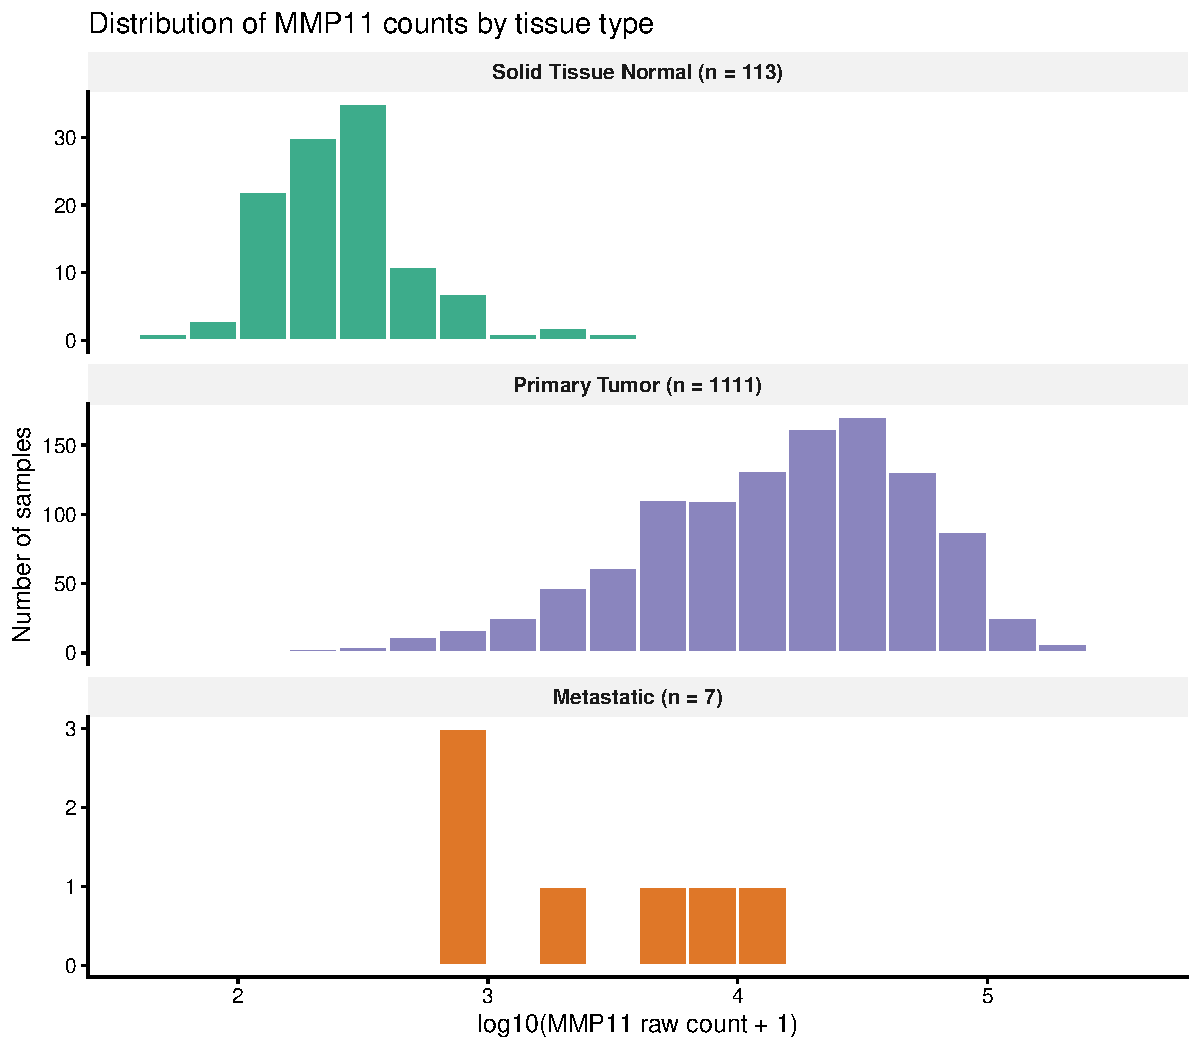
\includegraphics[width=0.9\textwidth]{mmp11_histogram.pdf}
\caption{Distribution of log-transformed
\textit{MMP11} raw counts in normal tissue, primary
tumor, and metastatic samples. Values are displayed
as $\log_{10}(\mathrm{raw\ count}+1)$.
Panels share the same horizontal scale but use
different vertical scales because the groups
have different sample sizes.}
\label{fig:mmp11-histogram}
\end{figure}

The primary tumor distribution was shifted toward
higher counts compared with normal tissue, although
the groups overlapped. Primary tumors also showed
a wider spread of log-transformed counts, indicating
variation among tumor samples.

The seven metastatic samples were spread across
an intermediate range relative to the normal and
primary tumor distributions. With so few metastatic
samples, the histogram provides limited information
about the shape of this group's distribution.

Because the panels use different vertical scales,
bar heights should be interpreted within each panel.
The shared horizontal scale allows comparison of
the locations and ranges of counts across tissue groups.

\clearpage
\subsection{Relationship between MMP11 and SCARA5 counts}

Figure~\ref{fig:gene-scatter} displays both genes'
log-transformed raw counts for each sample.
Following peer feedback, I highlighted the seven
metastatic samples as orange triangles to make
their positions easier to identify.

\begin{figure}[H]
\centering
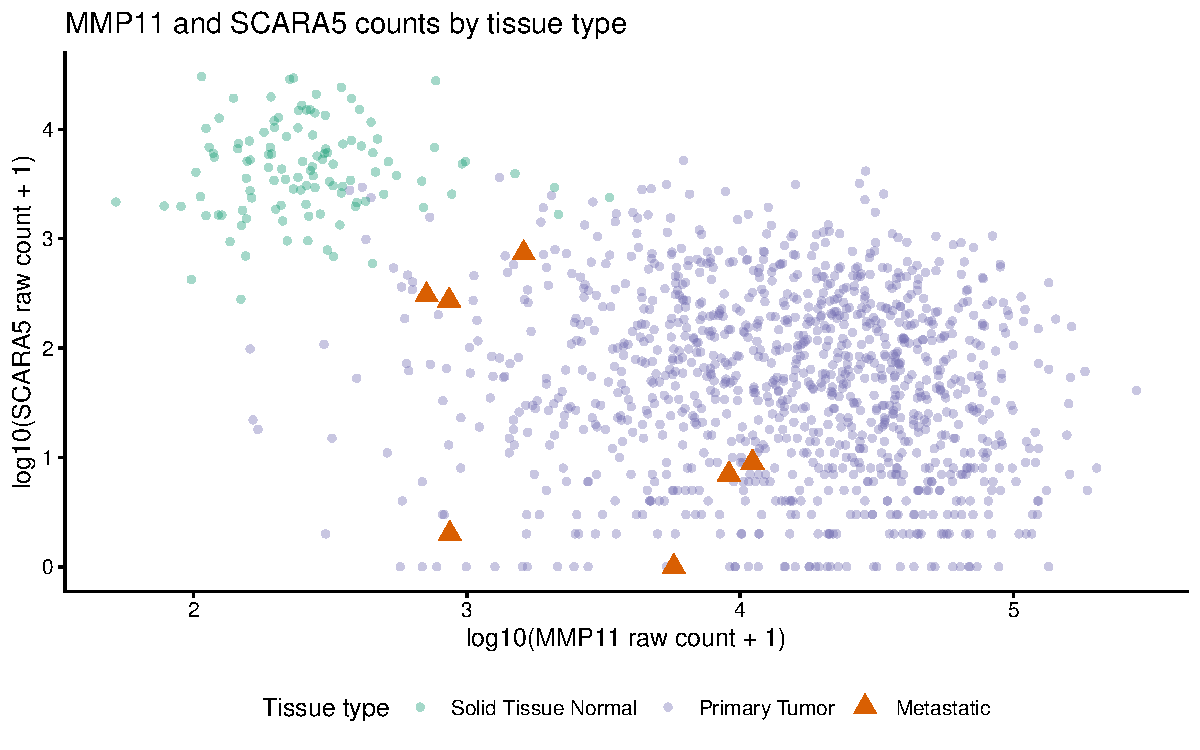
\includegraphics[width=\textwidth]{gene_scatter.pdf}
\caption{Relationship between log-transformed
\textit{MMP11} and \textit{SCARA5} raw counts.
Both axes use $\log_{10}(\mathrm{raw\ count}+1)$.
Each point represents one sample.
Normal tissue samples are green, primary tumors
are purple, and metastatic samples are highlighted
as orange triangles.}
\label{fig:gene-scatter}
\end{figure}

Normal tissue samples generally appeared toward
the upper left, with lower \textit{MMP11} counts
and higher \textit{SCARA5} counts. Primary tumors
generally appeared farther to the right and lower
on the plot, showing the opposite pattern.
The groups overlapped, and primary tumors showed
considerable variation.

The metastatic samples overlapped the broad range
occupied by primary tumors rather than forming
a clearly separate cluster. Their positions varied,
with some showing lower \textit{MMP11} counts than
most primary tumors. With only seven samples,
this observation remains descriptive.

The overall pattern suggests an inverse relationship
between the two genes across the combined dataset.
However, much of this pattern reflects differences
between tissue groups and does not establish that
one gene regulates the other.


\subsection{Comparison of counts across tissue types}

Figure~\ref{fig:gene-boxplots} summarizes the
log-transformed raw counts for both genes by
tissue type.

\begin{figure}[H]
\centering
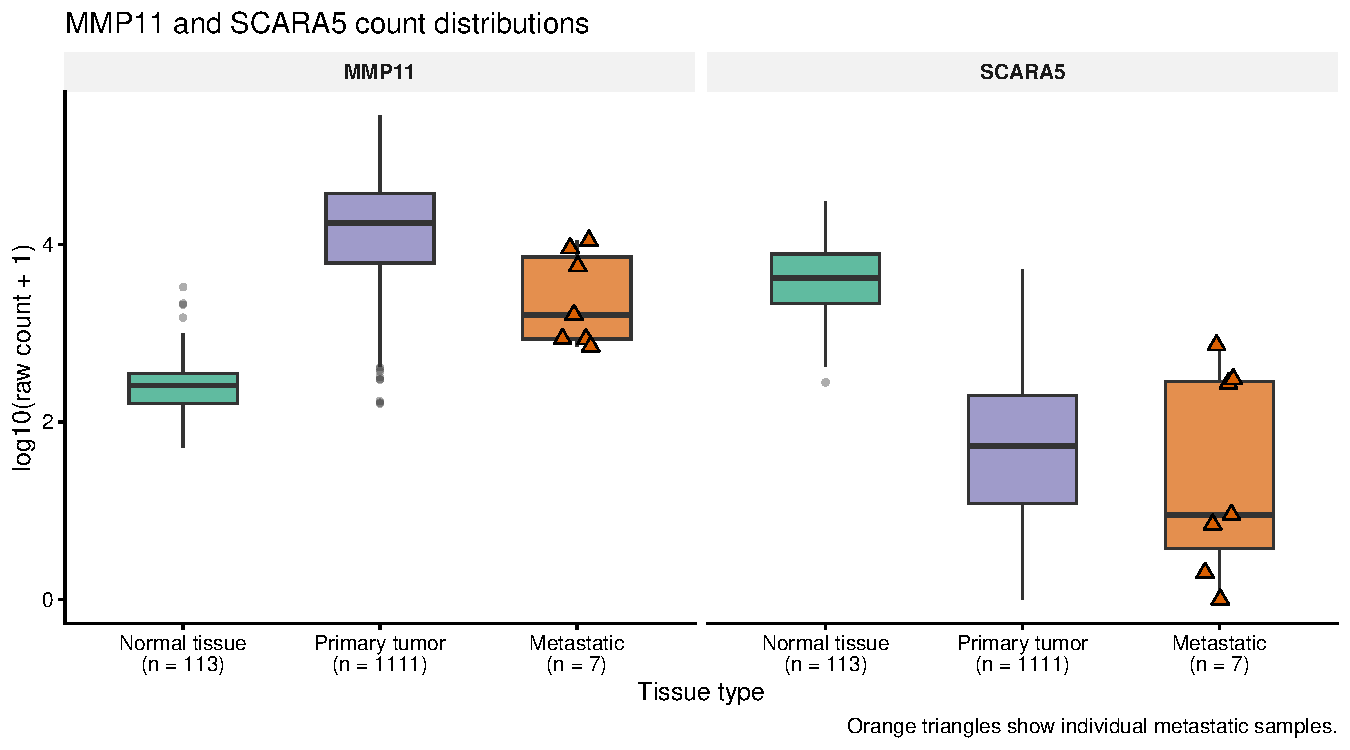
\includegraphics[width=\textwidth]{gene_boxplots.pdf}
\caption{Box plots of
$\log_{10}(\mathrm{raw\ count}+1)$ for
\textit{MMP11} and \textit{SCARA5} across tissue
groups. The central line represents the median,
and each box contains the middle 50\% of values.
Whiskers extend to the most extreme observations
within 1.5 times the interquartile range of the box.
Points beyond the whiskers are shown individually.
Orange triangles show the seven individual
metastatic samples.}
\label{fig:gene-boxplots}
\end{figure}

For \textit{MMP11}, primary tumors had a higher
median count than normal tissue. The middle 50\%
of values in these two groups were clearly separated,
although some individual samples overlapped.
The metastatic median fell between the normal
and primary tumor medians.

For \textit{SCARA5}, normal tissue had a higher
median count than either tumor group. Primary tumors
showed substantial variation, including samples with
zero counts. The metastatic median was lower than
both other groups, but the seven samples were
widely spread.

These plots reinforce the contrasting patterns
observed for the two genes. The individual
metastatic points also show how much variation
can be hidden by a summary box when the group
contains very few samples. These comparisons
describe the observed data and do not establish
statistical significance.


\subsection{Patterns across selected genes}

Figure~\ref{fig:gene-heatmap} shows the expression
patterns of 10 selected genes across all samples,
including \textit{MMP11} and \textit{SCARA5}.

\begin{figure}[H]
\centering
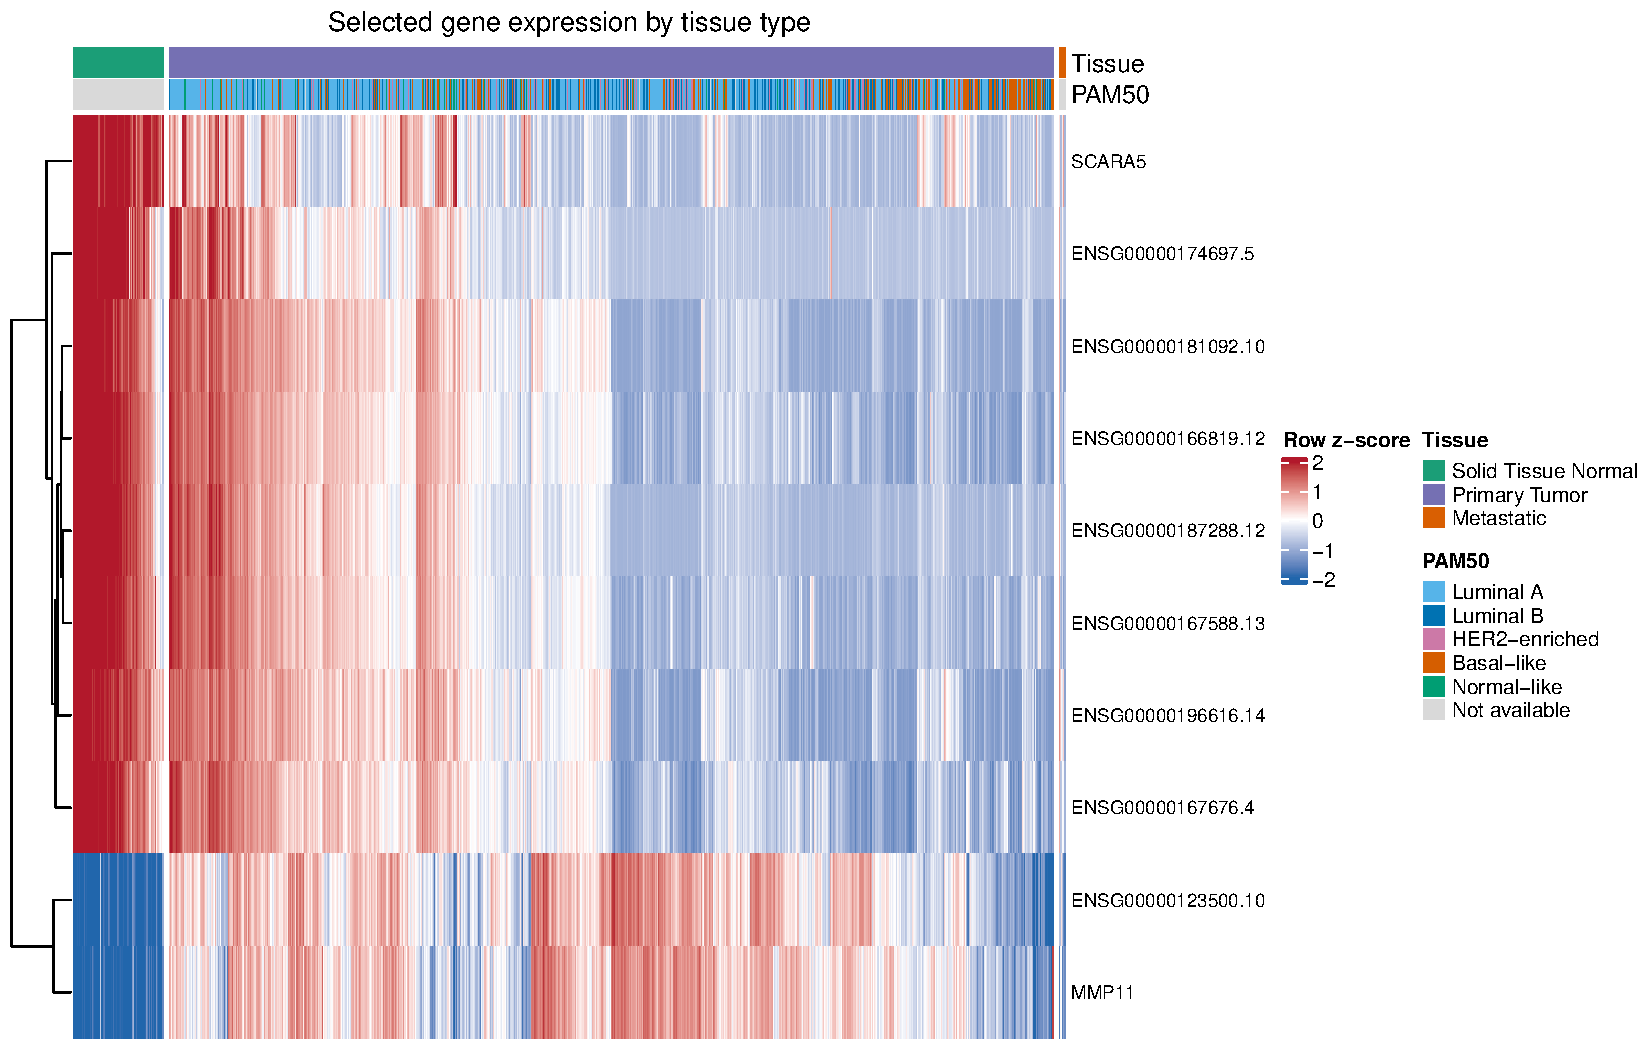
\includegraphics[width=\textwidth]{gene_heatmap.pdf}
\caption{Heatmap of 10 selected genes across
1,231 samples. Values were converted to CPM,
transformed using $\log_2(\mathrm{CPM}+1)$,
and standardized within each gene.
Red indicates values above that gene's mean
across samples, while blue indicates values below
its mean. Samples are grouped by tissue type
and clustered within each group.
Annotation bars identify tissue type and PAM50
molecular subtype; gray indicates unavailable
subtype information.}
\label{fig:gene-heatmap}
\end{figure}

Normal tissue samples generally showed higher
standardized values for \textit{SCARA5} and
several other selected genes, while
\textit{MMP11} showed lower values.
Many primary tumors showed the opposite pattern,
although there was considerable variation
within this group.

The PAM50 annotation provided context for
variation among primary tumors. Subtypes were
interspersed across the heatmap rather than
forming completely separate blocks.
The PAM50 category ``Normal-like'' describes
a molecular subtype and should not be confused
with the normal tissue sample group.

The metastatic samples form a narrow group
at the right edge because there were only seven.
Their small number limits interpretation
of a shared metastatic expression pattern.

Row standardization highlights relative variation
within each gene. Therefore, a red cell for one
gene does not necessarily represent a higher
absolute expression level than a blue cell
for another gene.

Because most genes were selected for large
observed differences between normal and primary
tumor samples, the contrasts in this heatmap
are expected and do not provide independent
validation of the gene-selection results.


\subsection{Cumulative distributions of gene counts}

Figure~\ref{fig:gene-ecdf} compares the cumulative
distributions of both genes across tissue groups.
At any horizontal-axis value, the height of a curve
shows the percentage of samples with values
at or below that value.

\begin{figure}[H]
\centering
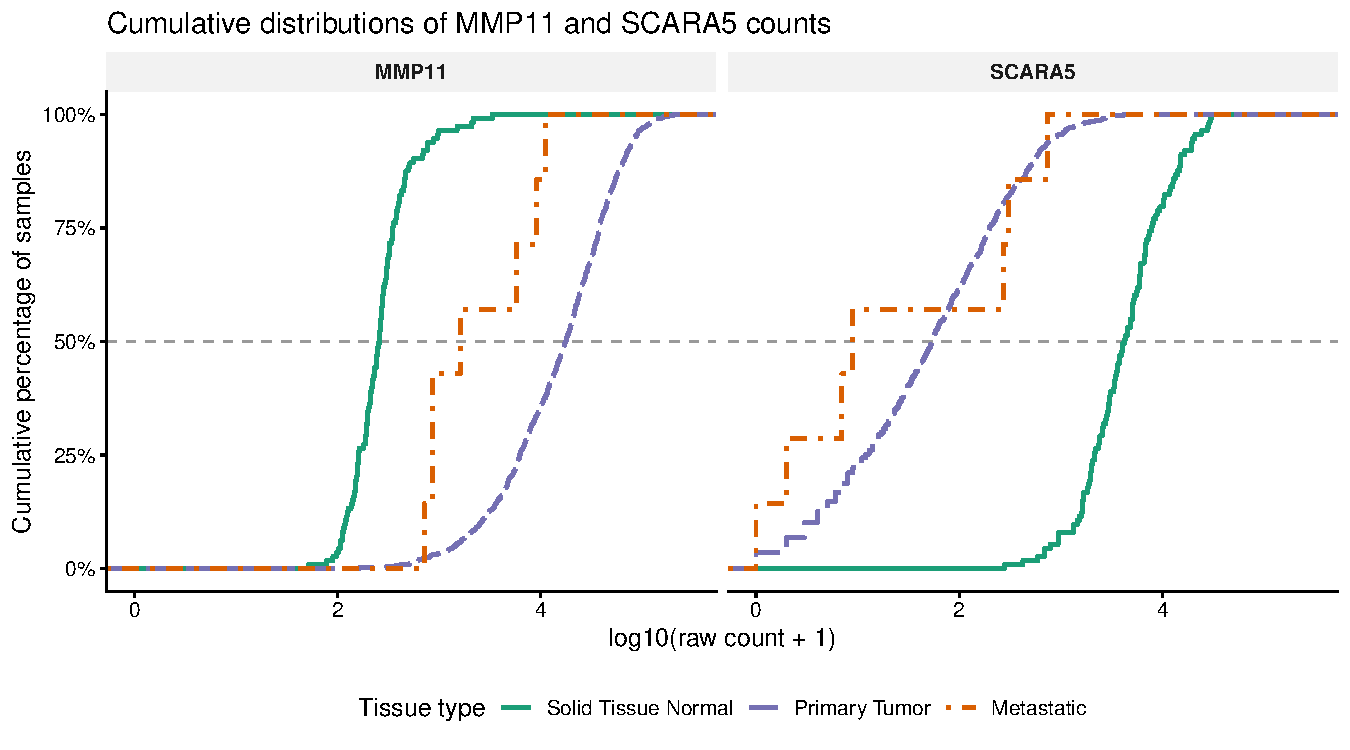
\includegraphics[width=\textwidth]{gene_ecdf.pdf}
\caption{Empirical cumulative distribution functions
of $\log_{10}(\mathrm{raw\ count}+1)$ for
\textit{MMP11} and \textit{SCARA5}, grouped by tissue
type. The dashed horizontal line marks 50\%,
allowing comparison of the group medians.
Each metastatic sample contributes approximately
14.3 percentage points to its group's curve,
producing larger steps than in the other groups.}
\label{fig:gene-ecdf}
\end{figure}

For \textit{MMP11}, the primary tumor curve was
shifted to the right of the normal tissue curve,
indicating generally higher counts in primary tumors.
The metastatic curve lay largely between them,
consistent with its intermediate median in
the box plot.

For \textit{SCARA5}, the normal tissue curve was
shifted to the right of both tumor groups,
indicating generally higher counts in normal tissue.
The metastatic and primary tumor curves crossed,
showing that their distributions could not be
described by a uniform shift in one direction.

Unlike a histogram, an ECDF does not require
a choice of bins. It also expresses each group's
distribution as a percentage, making groups
with different sample sizes easier to compare.
However, the metastatic curve remains based
on only seven observations and should be
interpreted cautiously.

\clearpage
\section{Conclusion}

This exploratory analysis identified contrasting
patterns for \textit{MMP11} and \textit{SCARA5}
across tissue groups. Primary tumors generally
had higher \textit{MMP11} counts and lower
\textit{SCARA5} counts than normal tissue.
These patterns were visible across several
complementary visualizations, although individual
samples overlapped and tumor samples showed
considerable variation.

In response to peer feedback, I highlighted
the seven metastatic samples in the scatter plot.
They overlapped the broad range occupied by
primary tumors rather than forming a clearly
separate cluster. Their small number limits
conclusions about metastatic tissue more broadly.

Several limitations affect interpretation.
The tissue groups differed greatly in sample size,
and some samples came from the same patients.
The histogram, scatter plot, box plots, and ECDFs
used log-transformed raw counts, which do not
adjust for differences in sequencing depth.
The heatmap used CPM, which accounts for sample
count totals but does not address all potential
technical or biological differences.

Finally, gene selection and visualization used
the same dataset. These findings therefore
describe observed patterns rather than providing
independent validation, evidence of causation,
or a validated diagnostic test. Further work
could use formal RNA-seq normalization,
account for patient relationships and relevant
covariates, and evaluate the selected genes
in an independent dataset.


% Start the references on a new page.
\clearpage

\begin{thebibliography}{9}

\bibitem{gdc}
National Cancer Institute.
\textit{TCGA-BRCA: Breast Invasive Carcinoma}.
Genomic Data Commons Data Portal.
\url{https://portal.gdc.cancer.gov/projects/TCGA-BRCA}.
Accessed October 18, 2026.

\bibitem{basset1990}
Basset, P., Bellocq, J. P., Wolf, C., et al. (1990).
A novel metalloproteinase gene specifically expressed
in stromal cells of breast carcinomas.
\textit{Nature}, 348, 699--704.
\url{https://doi.org/10.1038/348699a0}.

\bibitem{ulker2018}
Ulker, D., Ersoy, Y. E., Gucin, Z.,
Muslumanoglu, M., and Buyru, N. (2018).
Downregulation of SCARA5 may contribute to breast
cancer via promoter hypermethylation.
\textit{Gene}, 673, 102--106.
\url{https://doi.org/10.1016/j.gene.2018.06.036}.

\bibitem{ecdf}
ggplot2.
\textit{Compute empirical cumulative distribution:
stat\_ecdf}.
Package documentation.
\url{https://ggplot2.tidyverse.org/reference/stat_ecdf.html}.
Accessed October 18, 2026.

\end{thebibliography}

\end{document}